\documentclass[11pt]{article}

% LiveShark — minimal "premium product" style (printable, sober)

\usepackage[a4paper,margin=2.3cm]{geometry}

% Fonts: modern, readable, widely available in TeX Live
\usepackage{fontspec}
\setmainfont{DejaVu Serif}
\setsansfont{DejaVu Sans}

\usepackage{microtype}

% Color palette (subtle)
\usepackage{xcolor}
\definecolor{LSBlue}{HTML}{1A355E}
\definecolor{LSGray}{HTML}{F4F6F8}
\definecolor{LSMid}{HTML}{5B6675}

% Headings
\usepackage{titlesec}
\titleformat{\section}{\sffamily\bfseries\Large\color{LSBlue}}{\thesection}{0.8em}{}
\titleformat{\subsection}{\sffamily\bfseries\large\color{LSBlue}}{\thesubsection}{0.8em}{}
\titleformat{\subsubsection}{\sffamily\bfseries\normalsize\color{LSBlue}}{\thesubsubsection}{0.8em}{}
\titlespacing*{\section}{0pt}{2.0ex}{1.1ex}
\titlespacing*{\subsection}{0pt}{1.6ex}{0.9ex}

% Lists
\usepackage{enumitem}
\setlist[itemize]{leftmargin=*,topsep=0.4em,itemsep=0.25em}
\setlist[enumerate]{leftmargin=*,topsep=0.4em,itemsep=0.25em}

% Tables
\usepackage{booktabs}
\usepackage{tabularx}
\renewcommand{\arraystretch}{1.15}

% Links: NO red boxes
\usepackage[hidelinks]{hyperref}
\hypersetup{
  colorlinks=true,
  linkcolor=LSBlue,
  urlcolor=LSBlue,
  citecolor=LSBlue,
  pdfborder={0 0 0}
}

% Header/footer
\usepackage{fancyhdr}
\pagestyle{fancy}
\fancyhf{}
\renewcommand{\headrulewidth}{0.2pt}
\renewcommand{\footrulewidth}{0pt}
\fancyhead[L]{\sffamily\small\color{LSMid}\lsProjectTitle}
\fancyhead[R]{\sffamily\small\color{LSMid}\lsSpecStatus}
\fancyfoot[C]{\sffamily\small\color{LSMid}\thepage}

% Figures
\usepackage{graphicx}
\usepackage{caption}
\captionsetup{labelfont={sf,bf},textfont=sf,font=small}

% TikZ (for clean diagrams) — kept simple
\usepackage{tikz}
\usetikzlibrary{arrows.meta,positioning,shapes,fit}
\usepackage{adjustbox}

% Framed boxes for requirements/notes (subtle)
\usepackage[most]{tcolorbox}
\tcbset{
  colback=LSGray,
  colframe=LSBlue!35,
  arc=2mm,
  boxrule=0.4pt,
  left=1.4mm,right=1.4mm,top=1.0mm,bottom=1.0mm
}

% Project variables
\newcommand{\lsProjectTitle}{LiveShark — Specification}
\newcommand{\lsSpecStatus}{DRAFT}

% RFC 2119 keywords helpers (visual emphasis, not noisy)
\newcommand{\MUST}{\textbf{MUST}}
\newcommand{\MUSTNOT}{\textbf{MUST NOT}}
\newcommand{\SHOULD}{\textbf{SHOULD}}
\newcommand{\SHOULDNOT}{\textbf{SHOULD NOT}}
\newcommand{\MAY}{\textbf{MAY}}

% Requirement box (ID + priority)
\newtcolorbox{reqbox}[3]{title=\sffamily\bfseries #1 \hfill \sffamily #2, colback=LSGray, colframe=LSBlue!45}
% #1 = ID, #2 = Priority, #3 = (unused placeholder to allow future extensions)


\usepackage{csquotes}
\usepackage{biblatex}
\addbibresource{../common/references.bib}

\title{\sffamily\bfseries\color{LSBlue}LiveShark\\\large Specification (Printable PDF)}
\author{\sffamily Florian Keller}
\date{\sffamily Draft — \today}

\begin{document}
\maketitle
\vspace{-1.0em}

\begin{tcolorbox}
\textbf{Scope.} LiveShark is a \textbf{passive} analyzer for show-control networking (Art-Net, sACN). It focuses on
\textbf{offline PCAP analysis} with \textbf{DMX frame reconstruction}, \textbf{automatic conflict detection},
and \textbf{reproducible reports}.\\
\textbf{Audience.} Designed to be readable by \textbf{non-software specialists} (lighting technicians, integrators, QA).
\end{tcolorbox}

\tableofcontents
\newpage

\section{Terminology and conventions}

\subsection{Authoritative version and translation policy}
\textbf{Authoritative version (prevails).} The English specification in \texttt{spec/en} is the \emph{authoritative}
version: in case of discrepancy or incomplete translation, \textbf{the English version prevails}.\\
\textbf{Best-effort translation.} A French translation may exist in \texttt{spec/fr}. It is provided as a convenience and
\textbf{may lag behind}. When differences exist, the authoritative version prevails.

\subsection{Normative keywords}
The key words \MUST, \MUSTNOT, \SHOULD, \SHOULDNOT, and \MAY are to be interpreted as described in BCP 14
(RFC 2119 and RFC 8174). Only \textbf{UPPERCASE} usage is normative.


\subsection{Term note: \enquote{Live}}
In the project name, \enquote{Live} refers to \textbf{live entertainment / show control} (lighting networks), not to a guarantee
of real-time capture capability. Real-time capture is optional and may be introduced in later releases.

\subsection{Core terms}
\begin{tabularx}{\linewidth}{@{}l X@{}}
\toprule
\textbf{Term} & \textbf{Meaning} \\
\midrule
Packet & Network packet as captured in PCAP/PCAPNG. \\
Protocol message & Decoded application-layer unit (e.g., ArtDMX, sACN Data Packet). \\
DMX frame & Reconstructed DMX512 state (512 slots) for a universe at a given time. \\
Universe & Logical group of up to 512 DMX slots. \\
Source & Emitter identified by IP and, if applicable, protocol identity (e.g., sACN CID). \\
Flow & Unidirectional tuple (proto, src ip:port, dst ip:port). \\
\bottomrule
\end{tabularx}

\subsection{Acronyms}
\begin{tabularx}{\linewidth}{@{}l X@{}}
\toprule
\textbf{Acronym} & \textbf{Expanded form} \\
\midrule
DMX & Digital Multiplex (DMX512 / DMX512-A) \\
sACN & Streaming ACN (ANSI E1.31) \\
CID & Component Identifier (sACN source identifier) \\
PCAP & Packet Capture file format \\
FPS / PPS / BPS & Frames / Packets / Bytes per second \\
DoD & Definition of Done \\
\bottomrule
\end{tabularx}

\section{What LiveShark is (and is not)}

\subsection{Goals}
\begin{itemize}
  \item Offline analysis of PCAP/PCAPNG for Art-Net and sACN.
  \item DMX frame reconstruction (512 slots) and metrics (fps, pps/bps, jitter).
  \item Automatic detection of \textbf{conflicts} (multiple sources on same universe with overlap).
  \item Versioned, reproducible JSON reports for tickets, post-mortem, QA and CI.
\end{itemize}

\paragraph{Capture input (no Wireshark required).}
LiveShark \MUSTNOT{} require the Wireshark GUI application to operate.
For v0.1, captures are provided as PCAP/PCAPNG files produced by standard tools (e.g., \texttt{tcpdump} on Linux, \texttt{pktmon} on Windows, or any capture tool that exports PCAP/PCAPNG).
Live capture is a future objective and \MAY{} be added later via libpcap/Npcap (without changing the report schema).



\subsection{Offline-first strategy (product intent)}
LiveShark is designed as an \emph{offline-first} analyzer: early releases focus on post-mortem analysis of PCAP/PCAPNG captures
to maximize robustness, reproducibility, and ease of support. This is a deliberate engineering strategy, not a product limitation.
Live capture / online analysis is an explicit future objective and \MAY{} be implemented once the offline core is validated.

\textbf{Forward compatibility.} The core analysis pipeline \MUST{} be architected so that packet input can come from either:
(a) a file reader (PCAP/PCAPNG), or (b) a live capture source (future). No offline-only assumption \MUST{} be embedded in the
domain model (frames, conflicts, reports).



\subsection{Non-goals}
\begin{itemize}
  \item LiveShark is \textbf{not} a general-purpose packet analyzer (it does not replace Wireshark).
  \item LiveShark is \textbf{passive} by design: it does not transmit or inject traffic.
  \item ``Laser over IP'' starts as \textbf{generic UDP flow metrics only}; laser frame reconstruction is out of scope for v0.1.
\end{itemize}

\section{Architecture (conceptual)}
\begin{figure}[h]
\centering
\begin{adjustbox}{max width=\linewidth}
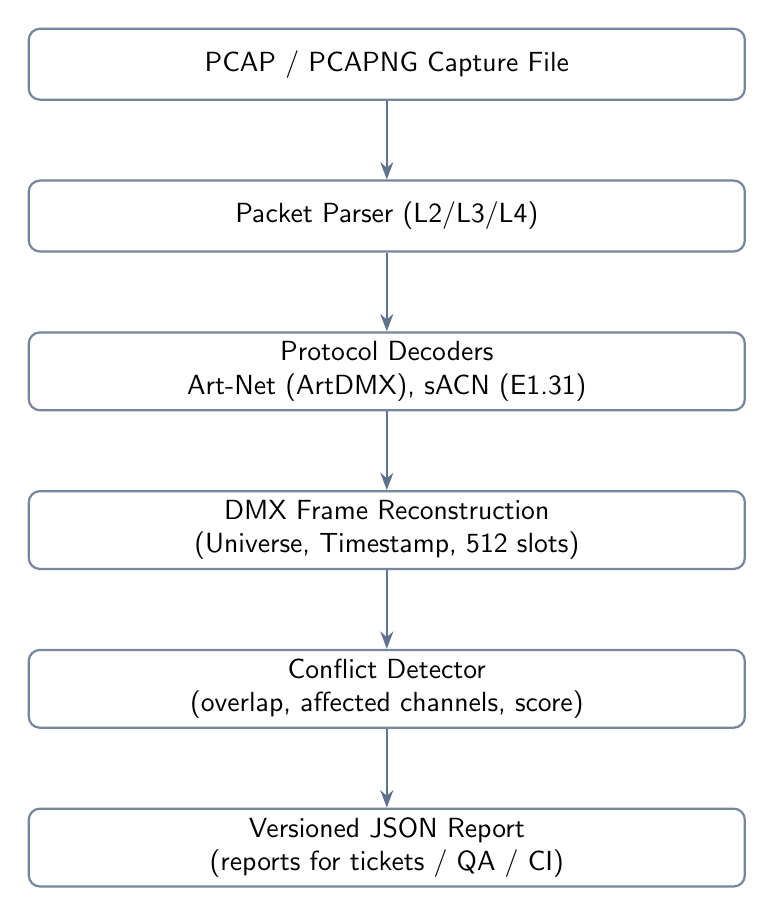
\begin{tikzpicture}[
  node distance=10mm,
  box/.style={rounded corners, draw=LSBlue!60, fill=white, thick, minimum width=0.75\linewidth, minimum height=9mm, align=center, font=\sffamily},
  arrow/.style={-{Stealth[length=2.2mm]}, thick, draw=LSBlue!70},
]
\node[box] (pcap) {PCAP / PCAPNG Capture File};
\node[box, below=of pcap] (parse) {Packet Parser (L2/L3/L4)};
\node[box, below=of parse] (decode) {Protocol Decoders \\ Art-Net (ArtDMX), sACN (E1.31)};
\node[box, below=of decode] (frame) {DMX Frame Reconstruction \\ (Universe, Timestamp, 512 slots)};
\node[box, below=of frame] (conf) {Conflict Detector \\ (overlap, affected channels, score)};
\node[box, below=of conf] (report) {Versioned JSON Report \\ (reports for tickets / QA / CI)};
\draw[arrow] (pcap) -- (parse);
\draw[arrow] (parse) -- (decode);
\draw[arrow] (decode) -- (frame);
\draw[arrow] (frame) -- (conf);
\draw[arrow] (conf) -- (report);
\end{tikzpicture}

\end{adjustbox}
\caption{Conceptual offline analysis pipeline (high level).}
\end{figure}

\section{Metrics (defaults)}
Unless otherwise stated:
\begin{itemize}
  \item \textbf{pps/bps window:} 1.0 s sliding window
  \item \textbf{fps window:} 5.0 s sliding window
  \item \textbf{jitter window:} 10.0 s sliding window (see metrics definition; concept reference: RFC 3550)
\end{itemize}

\section{Contractual requirements (extract)}
This document is a bootstrap spec: requirements are intentionally minimal at project start.


\begin{reqbox}{LS-ARCH-001}{P0}{}
The core \MUST{} expose a packet/event input abstraction so that analysis can be driven by:
(a) a PCAP/PCAPNG file reader (v0.1), and (b) a live capture source (future), without changing the domain model or report schema.
\end{reqbox}

\begin{reqbox}{LS-PROD-001}{P0}{}
LiveShark \MUSTNOT{} require the Wireshark GUI application. It \MUST{} accept PCAP/PCAPNG files produced by standard capture tools.
\end{reqbox}



\begin{reqbox}{LS-FR-001}{P0}{}
LiveShark \MUST ingest PCAP/PCAPNG files and enumerate UDP flows.
\end{reqbox}

\begin{reqbox}{LS-FR-010}{P0}{}
LiveShark \MUST decode Art-Net ArtDMX and reconstruct DMX frames (512 slots) per universe.
\end{reqbox}

\begin{reqbox}{LS-FR-011}{P0}{}
LiveShark \MUST decode sACN (E1.31) DMX data packets and reconstruct DMX frames per universe.
\end{reqbox}

\begin{reqbox}{LS-CONF-001}{P1}{}
LiveShark \MUST detect concurrent sources: two or more sources emitting on the same universe with overlap $> 1.0$ s.
\end{reqbox}

\begin{reqbox}{LS-REP-001}{P1}{}
LiveShark \MUST generate a versioned JSON report containing at least: capture summary, universes, sources, flows, and conflicts.
\end{reqbox}

\section{Licensing}
Code is licensed under \textbf{MIT OR Apache-2.0}. Documentation and specifications are licensed under \textbf{CC-BY-4.0}.

\section{Normative references}
\nocite{rfc2119,rfc8174,rfc3550,e1312018,artnet4}
\printbibliography

\end{document}
